\chapter{Funciones continuas}
\begin{comment}
\setcounter{section}{1}
\section{Definición de límite de una función}
La continuidad existe si existe  continuidad por la izquierda y por la derecha.

\begin{tcolorbox}
    \begin{def.}[Definición de entorno de un punto]
	Cualquier intervalo abierto que contenga un punto $p$ como su punto medio se denomina entorno de $p$.
    \end{def.}
\end{tcolorbox}

\textbf{Notación.-} Designemos los entornos con $N(p), N_1(p), N_2(p),$ etc. Puesto que un entorno $N(p)$ es un intervalo abierto simétrico respecto a $p$, consta de todos los números reales $x$ que satisfagan $p-r<x<p+r$ para un cierto $r>0$. El número positivo $r$ se llama radio del entorno. En lugar de $N(p)$ ponemos $N(p;r)$ si deseamos especificar su radio. Las desigualdades $p-r<x<p+r$ son equivalentes a $-r<x-p<r$, y a $|x-p|<r$. Así pues, $N(p;r)$ consta de todos los puntos $x$ , cuya distancia a $p$ es menor que $r$.\\
En la definición que sigue suponemos que $A$ es un número real y que $f$ es una función definida en un cierto entorno de un punto $p$ (excepción hecha acaso del mismo $p$). La función puede estar definida en $p$ pero esto no interviene en la definición.\\

\begin{tcolorbox}
    \begin{def.}[Definición de límite de una función]
	El simbolismo $$\lim_{x\to p}f(x)=A\qquad [\mbox{o}\; {f(x)\to A}\quad {x\to p}]$$
	significa que para todo entorno $N_1(A)$ existe un cierto entorno $N_2(p)$ tal que 
	\begin{center}
	    $f(x)\in N_1(A)$ siempre que $x\in N_2(p)$ y $x\neq p$
	\end{center}
	\vspace{0.3cm}
	El entorno $N_1(A)$ se cita en primer lugar, e indica cuán próximo queremos que sea $f(x)$ a su límite $A$. El segundo entorno, $N_2(p)$, nos indica lo próximo que debe estar $x$ de $p$ para que $f(x)$ sea interior al primer entorno $N_1(p)$. El entorno $N_2(p)$ dependerá del $N_1(A)$ elegido. Un entorno $N_2(p)$ que sirva para un $N_1(A)$ determinado servirá también, naturalmente, para cualquier $N_1(A)$ mayor, pero puede no ser útil para todo $N_1(A)$ más pequeño.\\
	Decir que $f(x)\in N_1(A)$ es equivalente a la desigualdad $|f(x)-A|<\epsilon$ y poner que $x\in N_2(p),\; x\neq p$ es lo mismo que escribir $0<|x-p|<\delta$. Por lo tanto, la definición de límite puede también expresarse así:\\\\
	El símbolo $\lim\limits_{x\to p}f(x)=A$ significa que para todo $\epsilon > 0$, existe un $\delta >0$ tal que $$|f(x)-A|<\epsilon \quad \mbox{siempre que}\quad 0<|x-p|<\delta.$$
    \end{def.}
\end{tcolorbox}

Observamos que las tres desigualdades,

\begin{center}
    $\lim\limits_{x\to p}f(x)=A$, $\lim\limits_{x\to p}(f(x)-A)=0$, $\lim\limits_{x\to p}[f(x)-A]=0$
\end{center}

Son equivalentes. También son equivalentes las desigualdades,
    
\begin{center}
    $\lim\limits_{x\to p} f(x)=A,$ $\lim\limits_{h\to 0}f(p+h)=A.$
\end{center}

Todas estas se derivan de la definición de límite.\\
\begin{tcolorbox}
    \begin{def.}[Límites laterales]
	Los límites laterales pueden definirse en forma parecida. Por ejemplo, si ${f(x)\to A}$ cuando ${x\to p}$ con valores mayores que $p$, decimos que $A$ es el límite por la derecha de $f$ en $p$, indicamos esto poniendo
	$$\lim_{x\to p^+}f(x)=A.$$
	En la terminología de los entornos esto significa que para todo entorno $N_1(A),$ existe algún entorno $N_2(p)$ tal que 
	$$f(x)\in N_1(A)\; \mbox{siempre que}\; x \in N_2(p)\quad \mbox{y}\quad x>p.$$
	Los límites a la izquierda, que indican poniendo ${x\to p^-}$, se definen del mismo modo restringiendo $x$ a valores menores que $p$.
    \end{def.}
\end{tcolorbox}

\section{Definición de continuidad de una función}

\begin{tcolorbox}
    \begin{def.}[Definición de continuidad de una función en un punto]
	Se dice que una función $f$ es continua en un punto $p$ si 
	\begin{enumerate}[\bfseries a)]
	    \item $f$ está definida en $p$, y
	    \item $\lim\limits_{x\to p}f(x)=f(p)$.
	\end{enumerate}
	Esta definición también puede formularse con entornos. Una función $f$ es continua en $p$ si para todo entorno $N_1[f(p)]$ existe un entorno $N_2(p)$ tal que 
	$$f(x)\in N_1[f(p)]\; \mbox{siempre que}\; x \in N_2(p).$$
	Puesto que $f(p)$ pertenece siempre a $N_1[f(p)]$, no se precisa la condición $x\neq p$.\\\\
	Especificando los radios de los entornos, la definición de continuidad puede darse como sigue:
	\begin{center}
	    $|f(x)-f(p)|<\epsilon$ siempre que $|x-p|<\delta$.
	\end{center}
    \end{def.}
\end{tcolorbox}

\section{Teoremas fundamentales sobre límites. Otros ejemplos de funciones continuas.}

%-------------------- teorema 3.1 --------------------------
\begin{tcolorbox}
    \begin{teo}
	Sean $f$ y $g$ dos funciones tales que 
	$$\lim_{x\to p} f(x)=A,\qquad \lim_{x\to p}g(x)=B$$
	Se tiene entonces
	\begin{enumerate}[\bfseries (i)]
	    \item $\lim\limits_{x\to p} [f(x)+g(x)]=A+B$,
	    \item $\lim\limits_{x\to p} [f(x)-g(x)]=A-B$,
	    \item $\lim\limits_{x\to p} f(x)\cdot g(x) = A\cdot B$,
	    \item $\lim\limits_{x\to p} \dfrac{f(x)}{g(x)} = \dfrac{A}{B}\qquad \mbox{si}\; B\neq 0$.\\
	\end{enumerate}
	Las demostraciones estarán dadas en la sección 3.5.
    \end{teo}
\end{tcolorbox}


Observemos primero que las afirmaciones del teorema pueden escribirse en forma un poco distinta. Por ejemplo, (i) puede ponerse como sigue:
$$\lim_{x\to p}[f(x)+g(x)]=\lim_{x\to p}f(x) + \lim_{x\to p}g(x).$$\\
Es costumbre indicar por $f+g$, $f-g$, $f\cdot g$ y $f/g$ las funciones cuyos valores para cada $x$ son:
$$f(x)+g(x),\quad f(x)-g(x),\quad f(x)\cdot g(x),\quad y \quad f(x)/g(x).$$\\

\begin{teo}
    Sean $f$ y $g$ dos funciones continuas en un punto $p$. La suma $f+g$, la diferencia $f-g$,  el producto $f\cdot g$ y  $g(p)\neq 0$ siempre que $g(p)\neq 0$ son también continuas en $p$.\\\\
    Demostración.-\; Puesto que $f$ y $g$ son continuas en $p$, se tiene $\lim\limits_{x\to p} f(x)=f(p)$ y $\lim\limits_{x\to p}g(x)=g(p)$. Aplicando las propiedades para límites, dadas en el teorema 3.1, cuando $A=f(p)$ y $B=g(p)$, se deduce el teorema 3.2.\\\\
\end{teo}

El teorema que sigue demuestra que si una función $g$ está intercalada entre otras dos funciones que tienen el mismo límite cuando $x\to p,$ $g$ tiene también este límite cuando $x\to p.$\\\\

% -------------------- teorema 3.3 --------------------------
\begin{teo}[Principio de intercalación]
    Supongamos que $f(x)\leq g(x)\leq h(x)$ para todo $x\neq p$ en un cierto entorno $N(p)$. Supongamos también que 
    $$\lim_{x\to p}f(x)=\lim_{x\to p}h(x)=a.$$
    Se tiene entonces $\lim_{x\to p}g(x)=a.$\\\\
	Demostración.-\; Sean $G(x)=g(x)-f(x)$, y $H(x)=h(x)-f(x)$. Las desigualdades $f\leq g\leq h$ implican $0\leq g-f\leq h-f$ o
	$$0\leq G(x)\leq H(x)$$
	para todo $x\neq p$ en $N(p)$. Para demostrar el teorema, basta probar que $G(x)\to 0$ cuando $x\to p$, dado que $H(x)\to 0$ cuando $x\to p$.\\
	Sea $N_1(0)$ un entorno cualquier de $0$. Puesto que $H(x)\to 0$ cuando $x\to p,$ existe un entorno $N_2(p)$ tal que 
	\begin{center}
	    $H(x) \in N_1(0)$ siempre que $x\in N_2(p)$ y $x\neq p.$
	\end{center}
	    Podemos suponer que $N_2(p) \subseteq N(p)$. Entonces la desigualdad $0\leq G \leq H$ establece que $G(x)$ no está más lejos de $0$ si $x$ está en $N_2(p), x\neq p$. Por consiguiente $G(x)\in N_1(0)$ para tal valor $x$ y por tanto $G(x)\to 0$ cuando $x\to p$. La misma demostración es válida si todos los límites son límites a un lado.\\\\
\end{teo}

% -------------------- teorema 3.4 --------------------------
\begin{teo}[Continuidad de las integrales indefinidas]
    Supongamos que $f$ es integrable en $[a,x]$ para todo $x$ en $[a,b]$, y sea
    $$A(x)=\int_a^x f(t)\; dt$$
    Entonces la integral indefinida $A$ es continua en cada punto de $[a,b]$ (En los extremos del intervalo tenemos continuidad a un lado.)\\\\
	Demostración.-\; Elijamos $p$ en $[a,b]$. Hay que demostrar que $A(x)\to A(p)$ cuando $x\to p.$ Tenemos
	$$A(x)-A(p)=\int_p^x f(t)\; dt$$
	Puesto que $f$ está acotada en $[a,b]$, existe una constante $M>0$ tal que $-M\leq f(t)\leq M$ para $t$ en $[a,b]$. Si $x>p$, integramos esas desigualdades en el intervalo $[p,x]$ obteniendo
	$$\int_p^x -M \;dt \leq \int_p^x f(t)\; dt\leq \int_p^x M \; dt \quad \Longrightarrow \quad -M(x-p)\leq A(x)-A(p)\leq M(x-p).$$
	Si $x<p$, obtenemos las mismas desigualdades con $x-p$ sustituida por $p-x$. Por consiguiente, en uno u otro caso podemos hacer que $x\to p$ y aplicar el principio de intercalación encontrando que $A(x)\to A(p)$. Esto prueba el teorema. Si $p$ es un extremo de $[a,b]$, tenemos que hacer que $x\to p$ desde el interior del intervalo, con lo que los límites son a un lado.
\end{teo}


\section{Demostraciones de los teoremas fundamentales sobre límites}

Demostración de (i) y (ii). Puesto que las dos igualdades:

\begin{center}
    $\lim\limits_{x\to p}f(x)=A\;$ y $\;\lim\limits_{x\to p}[f(x)-A]=0$
\end{center}

son completamente equivalentes, y como se tiene

$$f(x)+g(x)-(A+B) = [f(x)-A]+[g(x)-B],$$

basta demostrar las igualdades (i) y (ii) del teorema cuando los límites de $A$ y $B$ son ambos cero.\\
Supóngase pues, que $f(x)\to 0$ y $g(x)\to 0$ cuando $x\to p$. Se demostrará en primer lugar que $f(x)+g(x)\to 0$ cuando $x\to p$. Para ello se tiene que probar que para cada $\epsilon > 0$ existe un $\delta>0$ tal que 

\begin{center}
    $|f(x)+g(x)|<\epsilon\; $ siempre que $\;0<|x-p|<\delta.$
\end{center}

Sea $\epsilon$ dado. Puesto que $f(x)\to 0$ cuando $x\to p$, exista un $\delta_1>0$ tal que 

\begin{center}
    $|f(x)|<\dfrac{\epsilon}{2}\;$ siempre que $\; 0<|x-p|<\delta_1.$
\end{center}

Análogamente, puesto que $g(x)\to 0$ cuando $x\to p$ existe un $\delta_2>0$ tal que:

\begin{center}
    $|g(x)|<\dfrac{\epsilon}{2}\;$ siempre que $\; 0<|x-p|<\delta_2.$
\end{center}

Si se indica por $\delta$ el menor de los dos números $\delta_1$ y $\delta_2$, entonces, ambas igualdades últimas son válidas si $0<|x-p|<\delta$, y por tanto, en virtud de la desigualdad triangular, se tiene:

$$|f(x)+g(x)|\leq |f(x)|+|g(x)|<\dfrac{\epsilon}{2}+\dfrac{\epsilon}{2}=\epsilon$$

Esto demuestra la proposición dada que, a su vez, demuestra (i). La demostración de (ii) es completamente análoga, salvo que en el último paso se emplea la desigualdad $|f(x)-g(x)|\leq |f(x)|+|g(x)|.$\\\\

Demostración de (iii). Supóngase que se ha demostrado (iii) en el caso particular en que uno de los límites es $0$. Entonces el caso general resulta fácilmente de este caso particular, como se deduce de la siguiente igualdad:
$$f(x)g(x)-AB = f(x)[g(x)-B]+B[f(x)-A].$$
El caso particular implica que cada término del segundo miembro tienda a $0$ cuando $x\to p$ y en virtud de la propiedad (i) la suma de los dos términos tiende también a $0$. Por tanto, basta sólo probar (iii) en el caso en que uno de los límites, por ejemplo $B$, sea $0$.\\
Supóngase que $f(x)\to A$ y $g(x)\to 0$ cuando $x\to p$. Se trata de probar que $f(x)\cdot g(x)\to 0$ cuando $x\to p.$ Para ello se ha de ver que dado un número positivo $\epsilon,$ existe un $\delta>0$ tal que 
\begin{center}
$|f(x)g(x)|<\epsilon\;$ siempre que $\;0<|x-p|<\delta.$
\end{center}

Puesto que $f(x)\to A$ cuando $x\to p$, existe un $\delta_1$ tal que 

\begin{center}
    $|f(x)-A|<1\;$ siempre que $\; 0<|x-p|<\delta_1.$
\end{center}

Para tal $x$, tenemos $|f(x)-A+A|\leq |f(x)-A|+|A|<1+|A|,$ y por tanto

$$|f(x)g(x)|=|f(x)||g(x)|<(1+|A|)|g(x)|.$$

Ya que $f(x)\to 0$ cuando $x\to p$, para todo $\epsilon > 0$ existe un $\delta_2$ tal que 

\begin{center}
$|g(x)|<\dfrac{\epsilon}{1+|A|}\;$ siempre que $\; 0<|x-p|<\delta_2.$
\end{center}

Por consiguiente, si llamamos $\delta$ al menor de los dos números $\delta_1$ y $\delta_2$ entonces las dos igualdades son válidas siempre que $0<|x-p|<\delta$ y para tal valor de $x$ deducimos 

\begin{center}
$|f(x)g(x)|<\epsilon\;$ siempre que $\;0<|x-p|<\delta.$
\end{center}

Lo que completa la demostración.\\\\

Demostración de (iv). Puesto que el cociente $f(x)/g(x)$ es el producto de $f(x)/B$ por $B/g(x)$ basta demostrar que $B/g(x)\to 1$ cuando $x\to p$ y luego aplicar (iii). Sea $h(x)=g(x)/B$, por lo que $h(x)\to 1$ cuando $x\to p$, y se quiere demostrar que $1/h(x)$ cuando $x\to p$.\\
Dado $\epsilon>0,$ se trata de ver si existe un $\delta>0$ tal que
\begin{center}
$\bigg|\dfrac{1}{h(x)}\bigg|<\epsilon\;$ siempre que $\; 0<|x-p|<\delta.$
\end{center}
La diferencia se puede escribir como sigue:
$$\bigg|\dfrac{1}{h(x)}-1\bigg|=\dfrac{|h(x)-1|}{|g(x)|}.$$
Puesto que $g(x)\to 1$ cuando $x\to p$ se puede elegir un $\delta>0$ tal que ambas desigualdades:
$$|h(x)-1|<\dfrac{\delta}{2}\quad \mbox{y}\quad |h(x)-1|<\dfrac{1}{2}.$$
se satisfagan siempre que $0<|x-p|<\delta$. La segunda de estas desigualdades implica $h(x)>\dfrac{1}{2}$ y por tanto $1/|h(x)|=1/h(x)<2$ para tales valores de $x$. Empleando este resultado en junto con la primera desigualdad, obtenemos 
$$\bigg|\dfrac{1}{h(x)}-1\bigg|=\dfrac{|h(x)-1|}{|g(x)|}.$$
Esto completa la demostración de (iv).\\

\section{Ejercicios}

En los ejercicios del 1 al 10, calcular los límites y explicar cuáles han sido los teoremas utilizados en cada caso.\\\\

\begin{enumerate}[\bfseries 1.]

    %-------------------- 1.
    \item $\lim\limits_{x\to 2}\dfrac{1}{x^2}.$\\\\
	Respuesta.-\; 
	$$\lim\limits_{x\to 2}\dfrac{1}{x^2} = \dfrac{\lim\limits_{x\to 2}1}{\lim\limits_{x\to 2}x^2} = \dfrac{1}{2^2}=\dfrac{1}{4}.$$

	Esto por el teorema 3.1 inciso (iv) y por el hecho de que el límite de una constante es la misma constante.\\\\

    %-------------------- 2.
    \item $\lim\limits_{x\to 0} \dfrac{25x^3+2}{75x^7-2}$\\\\
	Respuesta.-\; 
	$$\lim\limits_{x\to 0} \dfrac{25x^3+2}{75x^7-2}=\dfrac{\lim\limits_{x\to 0}25x^3+\lim\limits_{x\to 0}2}{\lim\limits_{x\to 0}75x^7-\lim\limits_{x\to 0}2} = \dfrac{0 + 2}{0-2}=-1.$$
	Por el teorema 3.1 incisos (i),(ii) y (iii).\\\\

    %-------------------- 3.
    \item $\lim\limits_{x\to 2}\dfrac{x^2-4}{x-2}$.\\\\
	Respuesta.-\; 
	$$\lim\limits_{x\to 2}\dfrac{x^2-4}{x-2} = \lim_{x\to 2}\dfrac{(x-2)(x+2)}{x-2}=\lim_{x\to 2}(x+2) = \lim_{x\to 2} x + \lim_{x\to 2}2 = 4.$$
	Esto por el teorema 3.1 inciso (1).\\\\

    %-------------------- 4.
    \item $\lim\limits_{x\to 1}\dfrac{2x^2-3x+1}{x-1}$.\\\\
	Respuesta.-\; 
	$$\lim\limits_{x\to 1}\dfrac{2x^2-3x+1}{x-1} = \lim_{x\to 1}\dfrac{(2x-1)(x-1)}{x-1}=\lim_{x\to 1} 2x - \lim_{x\to 1} 1 = 1.$$
	Esto por el teorema 3.1 inciso (1).\\\\

    %-------------------- 5.
    \item $\lim\limits_{h\to 0}\dfrac{(t+h)^2-t^2}{h}.$\\\\
	Respuesta.-\; 
	$$\lim\limits_{h\to 0}\dfrac{(t+h)^2-t^2}{h} = \lim_{h\to 0}\dfrac{t^2+2th+h^2-t^2}{h}=\lim_{h \to 0} (2t+h) = \lim_{h\to 0}2t + \lim_{h\to 0}h = 2t.$$
	Esto por el teorema 3.1 inciso (1).\\\\

    %-------------------- 6.
    \item $\lim\limits_{x\to 0}\dfrac{x^2-a^2}{x^2+2ax+a^2},\qquad a\neq 0$.\\\\
	Respuesta.-\; 
	$$\lim\limits_{x\to 0}\dfrac{x^2-a^2}{x^2+2ax+a^2} = \lim_{x\to 0}\dfrac{(x-a)(x+a)}{(x+a)^2}=\lim_{x\to 0}\dfrac{x-a}{x+a}=\dfrac{\lim\limits_{x\to 0}x-\lim\limits_{x\to 0}a}{\lim\limits_{x\to 0}x + \lim\limits_{x\to 0}a} = -1.$$
	Por el teorema 3.1 incisos (i),(ii) y (iii).\\\\

    %-------------------- 7.
    \item $\lim\limits_{a\to 0}\dfrac{x^2-a^2}{x^2+2ax+a^2},\qquad a\neq 0.$\\\\
	Respuesta.-\; 
	$$\lim\limits_{a\to 0}\dfrac{x^2-a^2}{x^2+2ax+a^2} = \lim_{a\to 0}\dfrac{(x-a)(x+a)}{(x+a)^2}=\lim_{a\to 0}\dfrac{x-a}{x+a}=\dfrac{\lim\limits_{a\to 0}x-\lim\limits_{a\to 0}a}{\lim\limits_{a\to 0}x + \lim\limits_{a\to 0}a} = 1.$$
	Por el teorema 3.1 incisos (i),(ii) y (iii).\\\\

    %-------------------- 8.
    \item $\lim\limits_{x\to a}\dfrac{x^2-a^2}{x^2+2ax+a^2},\qquad a\neq 0.$\\\\
	Respuesta.-\; 
	$$\lim\limits_{x\to a}\dfrac{x^2-a^2}{x^2+2ax+a^2} = \lim_{x\to a}\dfrac{(x-a)(x+a)}{(x+a)^2}=\lim_{x\to a}\dfrac{x-a}{x+a}=\dfrac{\lim\limits_{x\to a}x-\lim\limits_{x\to a}a}{\lim\limits_{x\to a}x + \lim\limits_{x\to a}a} = 0$$
	Por el teorema 3.1 incisos (i),(ii) y (iii).\\\\

    %-------------------- 9.
    \item $\lim\limits_{t\to 0} \tan t.$\\\\
	Respuesta.-\; 
	$$\lim\limits_{t\to 0} \tan t = 0.$$\\

    %-------------------- 10.
    \item $\lim\limits_{t\to 0}(\sen 2t + t^2 \cos 5t).$\\\\
	Respuesta.-\; 
	$$\lim\limits_{t\to 0}(\sen 2t + t^2 \cos 5t) = \lim_{t\to 0}\sen 2t + \lim_{t\to 0}t^2\cdot \lim_{t\to 0}\cos 5t = 0.$$
	Por el teorema 3.1 incisos (i) y (iii).\\\\

    %-------------------- 11.
    \item $\lim\limits_{x\to 0^+}\dfrac{|x|}{x}.$\\\\
	Respuesta.-\; Ya que $|x|=x$ para $x>0$, por lo tanto tenemos  
	$$\lim_{x\to 0^+}\dfrac{|x|}{x}=\lim_{x\to 0^+}\dfrac{x}{x}=1.$$\\

    %-------------------- 12.
    \item $\lim\limits_{x\to 0^-}\dfrac{|x|}{x}.$\\\\
	Respuesta.-\; Ya que $|x|=-x$ para $x<0$, por lo tanto tenemos  
	$$\lim_{x\to 0^-}\dfrac{|x|}{x}=\lim_{x\to 0^-}\dfrac{-x}{x}=-1.$$\\

    %-------------------- 13.
    \item $\lim\limits_{x\to 0^+}\dfrac{\sqrt{x^2}}{x}.$\\\\
	Respuesta.-\; Para $x>0$ tenemos $\sqrt{x^2}=|x|=x$ entonces,
	$$\lim_{x\to 0^+}\dfrac{\sqrt{x^2}}{x}=\lim_{x\to 0^+} \dfrac{x}{x}=1.$$\\

    %-------------------- 14.
    \item $\lim\limits_{x\to 0^-}\dfrac{\sqrt{x^2}}{x}.$\\\\
	Respuesta.-\; Para $x<0$ tenemos $\sqrt{x^2}=|x|=-x$ entonces,
	$$\lim_{x\to 0^-}\dfrac{\sqrt{x^2}}{x}=\lim_{x\to 0^-} \dfrac{-x}{x}=-1.$$\\

	Utilizar la relación $\lim\limits_{x\to 0}(\sen x)/x$ para establecer las igualdades de los Ejercicios del 15 al 20.\\\\

    %-------------------- 15.
    \item $\lim\limits_{x\to 0}\dfrac{\sen 2x}{x}=2.$\\\\
	Respuesta.-\; Sea $\sen(2x) = 2\sen x \cos x$ entonces 
	$$\dfrac{\sen 2x}{x} = \dfrac{2\sen x \cos x}{x} = 2\cos x\left(\dfrac{\sen x}{x}\right)$$
	de donde 
	$$\lim_{x\to 0}\dfrac{\sen 2x}{x}=\lim_{x\to 0}\left(2\cos x \dfrac{\sen x}{x}\right) = \lim_{x\to 0}2\cdot \lim_{x\to 0}\cos x \cdot \lim_{x\to 0}\dfrac{\sen x}{x} = 2.$$\\

    %-------------------- 16.
    \item $\lim\limits_{x\to 0}\dfrac{\tan 2x}{\sen x}=2.$\\\\
	Respuesta.-\; Ya que $\tan2x = \dfrac{\sen 2x}{\cos 2x}$ entonces,
	$$\lim_{x\to 0}\dfrac{\tan 2x}{\sen x} = \lim_{x\to 0} \dfrac{\sen 2x}{\cos 2x \sen x} = \lim_{x\to 0} \dfrac{2\sen x \cos x}{\cos 2x \sen x}=\lim_{x\to 0} \dfrac{2\cos x}{\cos 2x}=2.$$\\

    %-------------------- 17.
    \item $\lim\limits_{x\to 0}\dfrac{\sen 5x}{\sen x}=5.$\\\\
	Respuesta.-\; Primeramente tenemos,
	$$\lim_{x\to 0}\dfrac{\sen 5x}{\sen x}=\lim_{x\to 0}\left[\left(\dfrac{\sen x}{x}\right)\left(\dfrac{\sen 5x}{\sen x}\right)\right]=\lim_{x\to 0}\dfrac{\sen 5x}{x}.$$
	Luego usando la formula $\sen(x+y)=\sen x \cos y + \cos x \sen y$ obtenemos,
	$$\begin{array}{rcl}
	    \lim\limits_{x\to 0}\dfrac{\sen 5x}{x}&=&\lim\limits_{x\to 0}\dfrac{\sen(4x+x)}{x}\\\\
						  &=&\lim\limits_{x\to 0}\dfrac{\sen 4x \cos x + \sen x \cos 4x}{x}\\\\
						  &=&\lim\limits_{x\to 0}\left(\dfrac{2\sen 2x \cos 2x \cos x}{x}+\dfrac{\sen x}{x}\cos 4x\right)\\\\
						  &=&\lim\limits_{x\to 0}\left(\dfrac{\sen 2x}{x}2\cos 2x \cos x + \dfrac{\sen x}{x}\cos 4x\right)\\\\
	\end{array}$$
	pero sabemos que $\lim\limits_{x\to 0}\dfrac{\sen 2x}{x}=2$, así 
	$$\lim_{x\to 0}\dfrac{\sen 5x}{\sen x}=\lim\limits_{x\to 0}\left(\dfrac{\sen 2x}{x}2\cos 2x \cos x + \dfrac{\sen x}{x}\cos 4x\right)=2\cdot 2 + 1\cdot 1 = 5.$$\\\\

    %-------------------- 18.
    \item $\lim\limits_{x\to 0}\dfrac{\sen 5x - \sen 3x}{x}=2.$\\\\
	Respuesta.-\; Sabemos por ejercicios anteriores que
	$$\lim_{x\to 0}\dfrac{\sen 5x}{x}=5,\qquad \mbox{y} \qquad \lim_{x\to 0}\dfrac{\sen 2x}{x}=2$$
	entonces 
	$$\begin{array}{rcl}
	    \lim\limits_{x\to 0}\dfrac{\sen 3x}{x}&=&\lim\limits_{x\to 0} \dfrac{\sen (2x+x)}{x}\\\\
						  &=&\lim\limits_{x\to 0}\dfrac{\sen 2x \cos x + \sen x \cos 2x}{x}\\\\
						  &=&\lim\limits_{x\to 0}\left(\dfrac{\sen 2x}{x}\cos x + \dfrac{\sen x}{x}\cos 2x\right)\\\\
	\end{array}$$
	por lo tanto
	$$\lim_{x\to 0}\dfrac{\sen 3x}{x}=2+1=3$$
	Así, por el teorema 3.1(ii),
	$$\begin{array}{rcl}
	    \lim\limits_{x\to 0}\dfrac{\sen 5x-\sen 3x}{x}&=&\lim\limits_{x\to 0}\left(\dfrac{\sen 5x}{x}-\dfrac{\sen 3x}{x}\right)\\\\
	    &=&\lim\limits_{x\to 0}\dfrac{\sen 5x}{x}-\lim\limits_{x\to 0}\dfrac{\sen 3x}{x}\\\\
	    &=&5-3\\\\
	    &=&2.\\\\
	\end{array}$$

    %-------------------- 19.
    \item $\lim\limits_{x\to a}\dfrac{\sen x - \sen a}{x-a}=\cos a.$\\\\
	Respuesta.-\; Por el teorema 2.3 (g) sabemos que 
	$$\sen a - \sen b = 2\sen \dfrac{a-b}{2} \cos \dfrac{a+b}{2}$$
	de donde 
	$$\lim_{x\to a}\dfrac{sen x-\sen a}{x-a}=\lim_{x\to a}\dfrac{2\sen \dfrac{x-a}{2}\cos \dfrac{x+a}{2}}{x-a} = \lim_{x\to a}\left(\dfrac{\sen \dfrac{x-a}{2}}{\dfrac{x-a}{2}}\cos \dfrac{x+a}{2}\right)$$
	pero,
	$$\lim_{x\to a}\dfrac{\sen \dfrac{x-a}{2}}{\dfrac{x-a}{2}}=\lim_{y\to 0}\dfrac{\sen y}{y}=1,\qquad \mbox{ya que, } \;y=\dfrac{x-a}{2} \; \mbox{ e } \; y\to 0 \;\mbox{ como }\; x\to a.$$
	así,
	$$\lim_{x\to a}\dfrac{\dfrac{x-a}{2}}{\dfrac{x-a}{2}}\cos \dfrac{x+a}{2}=\lim_{x\to a}\dfrac{x+a}{2}=\cos a.$$


    %-------------------- 20.
    \item $\lim\limits_{x\to 0}\dfrac{1-\cos x}{x^2}=\dfrac{1}{2}.$\\\\
	Respuesta.-\; Sea,
	$$\lim_{x\to 0}\dfrac{1-\cos x}{x^2}=\lim_{x\to 0} \dfrac{(1-\cos x)(1+\cos x)}{x^2(1+\cos x)}=\lim_{x\to 0}\dfrac{1-\cos^2 x}{x^2(1+\cos x)}$$
	Luego, ya que $\cos^2x+\sen^2 x = 1 \; \Longrightarrow \; 1-\cos^2x = \sen^2x,$ entonces
	$$\begin{array}{rcl}
	    \lim\limits_{x\to 0}\dfrac{1-\cos^2 x}{x^2(1+\cos x)}&=&\lim\limits_{x\to 0}\left(\dfrac{\sen^2 x}{x}\cdot \dfrac{1}{1+\cos x}\right)\\\\
								 &=&\lim\limits_{x\to 0}\left[\left(\dfrac{\sen x}{x}\right)^2 \dfrac{1}{1+\cos x}\right]\\\\
								 &=&\lim\limits_{x\to 0}\left[\dfrac{\sen x}{x}\cdot \dfrac{\sen x}{x}\cdot \dfrac{1}{1+\cos x}\right]\\\\
								 &=&\lim\limits_{x\to 0}\dfrac{1}{1+\cos x}\\\\
								 &=&\dfrac{1}{2}.\\\\


	\end{array}$$

    %-------------------- 21.
    \item Demostrar que $\lim\limits_{x\to 0}\dfrac{1-\sqrt{1-x^2}}{x^2}=\dfrac{1}{2}.$\\\\
	Demostración.-\; Multiplicando por el límite dado por $1+\sqrt{1-x^2}$ tenemos,
	$$\begin{array}{rcl}
	    \lim\limits_{x\to 0}&=&\lim\limits_{x\to 0}\dfrac{1-(1-x^2)}{x^2(1+\sqrt{1-x^2})}\\\\
				&=&\lim\limits_{x\to 0}\dfrac{x^2}{x^2(1+\sqrt{1-x^2})}\\\\
				&=&\lim\limits_{x\to 0}\dfrac{1}{1+\sqrt{1-x^2}}\\\\
				&=&\dfrac{1}{2}\\\\\
	\end{array}$$

    %-------------------- 22.
    \item Una función $f$ está definida como sigue:
    $$f(x)=\left\{\begin{array}{rcl}
	\sen x & \mbox{si} & x\leq c,\\
	ax+b & \mbox{si} & x>c,\\
    \end{array}\right.$$
    siendo $a,b,c$ constantes. Si $b$ y $c$ están dados, hallar todos los valores de $a$ (si existe alguno) para los que $f$ es continua en el punto $x=c$.\\\\
	Respuesta.-\; Por definición de continuidad, de una función en un punto, conocemos que $f$ es continua en $x=c$ el cual significa que $f$ está definida en $c$ y $\lim\limits_{x\to c} f(x)=f(c)$.\\
	Ya que $\sen x$ y $ax+b$ son definidos para todo $x\in \mathbb{R}$, conocemos que $f$ es conocida en $x=c$ para todo $c\in \mathbb{R}$. Entonces podemos encontrar valores de $a$ tal que 
	$$\lim_{x\to c}f(x)=f(c).$$
	Por la definición de $f$, sabemos que
	$$f(c)=\sen c$$
	Entonces, evaluamos el limite en $x\to c$ a través de valores mayores que $c$ (ya que el límite en $x\to c$ a través de valores menos que $c$ es $f(c)$ ya que $\sen x$ es una función continua y para valores menores que $c,$ $f(x)=\sen x$),
	$$\lim_{x\to c^+}f(x)=\lim_{x\to c^+} ax+b=ac+b$$
	y por lo tanto, para que $f$ sea continua en $c$ debemos tener,
	$$ac+b=\sen c\; \Longrightarrow\; b=0,\; \mbox{ y } a \mbox{ es arbitrario}.$$\\

    %-------------------- 23.
    \item Resolver el ejercicio 22 si $f$ se define de este modo:
    $$f(x)=\left\{\begin{array}{rcl}
	2\sen x & \mbox{si} & x\leq c,\\
	ax^2+b & \mbox{si} & x>c,\\
    \end{array}\right.$$
	Respuesta.-\; Por la definición de continuidad, conocemos que $f$ es continua en $x=c$ el cual significa que $f(c)$ es definida y $\lim\limits_{x\to c}f(x)=f(c)$. Ya que $2\cos x$ y $ax^2+b$ está definida para todo $x\in \mathbb{R}$, conocemos que $f$ es definida para todo $c\in \mathbb{R}$. Entonces para demostrar que es continua debemos demostrar
	$$\lim_{x\to c}f(x)=f(c).$$
	De la definición de $f$ sabemos 
	$$f(c)=2\cos c.$$
	Entonces, tomando el límite como $x$ se aproxima a $c$ por la derecha (ya que $\lim\limits_{x\to c^-} f(x)=f(c)$,  $2\cos x$ es continua y $f(x)=2\cos x$ cuando $x$ se aproxima a $c$ por la izquierda),
	$$\lim_{x\to c^+}f(x)=\lim_{x\to c^+} ax^2+b=ac^2+b.$$
	Así, debemos tener
	$$ac^2+b=2\cos c \; \Longrightarrow \; a=\dfrac{2\cos -b}{c^2} \mbox{ si } c\neq 0.$$
	Si $c=0$ entonces,
	$$ac^2+b=2\cos c \; \Longrightarrow \; b=2\, \mbox{ y } a \mbox{ es arbitrario}.$$\\

    %-------------------- 24.
    \item ¿En qué punto son funciones continuas la tangente y la cotangente?.\\\\
	Respuesta.-\; Sea $$\tan x = \dfrac{\sen x}{\cos x}$$
	y $\sen x,\, \cos x$ son continuas para todo los número reales de donde sabemos por el teorema 3.2 que $\tan x$ es continua en todas partes, por lo que $\cos x$ no es cero. Probamos que 
	$$\cos x=0 \; \Longleftrightarrow \; x=\dfrac{\pi}{2}+n\pi,\quad n\in \mathbb{Z}.$$
	por lo que $\tan x$ es continuo para 
	$$\lbrace x\in \mathbb{R} | x\neq \dfrac{\pi}{2}+n\pi,\; n\in \mathbb{Z} \rbrace$$
	Similarmente 
	$$\cot x = \dfrac{\cos x}{\sen x}$$
	 y por el teorema 3.2 tenemos que $\cot x$ es continua en todo lugar donde $\sen x$ no sea cero. Luego probamos que,
	 $$\sen x = 0\; \Longleftrightarrow \; x=n\pi \quad n  \in \mathbb{Z}.$$
	 Por lo tanto, $\cot x$ es continua para 
	 $$\lbrace x\in \mathbb{R} | x\neq n\pi, \; n \in mathbb{R}\rbrace.$$\\\\

    %-------------------- 25.
    \item Sea $f(x)=(\tan x/x)$ si $x\neq 0$. Esbozar la gráfica de $f$ correspondientes a los intervalos semiabiertos $[-\frac{1}{4}\pi,0]$. ¿Qué le ocurre a $f(x)$ cuando $x\to 0$? ¿Puede definirse $f(0)$ de modo que $f$ se haga continua en $0$?.\\\\
	Respuesta.-\; 
	    \begin{center}
		\begin{tikzpicture}
		\begin{axis}[scale=.7,draw opacity = .5, style={
		  domain=-1/4*pi:0,samples=100,smooth}, 
		  axis x line=center, % no box around the plot, only x and y axis
		  axis y line=center, % the * suppresses the arrow tips
		  ylabel = {$f(x)$},
		  xlabel = {$x$},
		  xlabel style={below right},
		  ylabel style={above left},
		  xmin=-1/4*pi,xmax=0,ymin=0,ymax=1.5,
		  enlargelimits=upper] % extend the axes a bit to the right and top
		  \addplot[black,opacity=1]{tan(deg(x))/x};
		\end{axis}
	    \end{tikzpicture}
	    \end{center}
	    \vspace{.5cm}

	    Tenemos que,
	    $$\begin{array}{rcl}
		\lim\limits_{x\to 0}\dfrac{\tan x}{x}&=&\lim\limits_{x\to 0}\dfrac{\sen x}{x\cos x}\\\\
						     &=&\lim\limits_{x\to 0}\left[\left(\dfrac{\sen x}{x} \right)\cos x\right]\\\\
						     &=&\lim\limits_{x\to 0}\cos x\\\\
						     &=&1.\\\\
	    \end{array}$$
	    ya que $f(x)=\dfrac{\tan x}{x}$ no está definida en cero entonces no es una función continua. Sin embargo, dado que el límite existe, podríamos redefinir $f$ por:
	    $$f(x)=\left\{\begin{array}{rcl}
		\dfrac{\tan x}{x}&\mbox{si}&x\neq 0\\\\
		1&\mbox{si}&x = 0\\\\
	    \end{array}\right.$$
	    \vspace{.5cm}

    %-------------------- 26.
	\item Este ejercicio ofrece otra demostración de la continuidad de las funciones seno y coseno. a) La desigualdad $|\sen x|<|x|$, válida para $0<|x|<\frac{1}{2}\pi$, fue demostrada en el ejercicio 34 de la sección 2.8. Utilizarla para demostrar que la función seno es continua en $0$. b) Hacer uso de la parte a) y de la identidad $\cos 2x = 1-2\sen^2 x$ para demostrar la continuidad del coseno en $0$.\\\\
	    Demostración.-\; Demostraremos primeramente que $\lim\limits_{x\to 0}\sen x = \sen 0 = 0$.\\
	    Para todo $\epsilon>0$ existe un $\delta >0$ tal que $|\sen x|<\epsilon$ entonces $|x|<\delta$. Sea $\delta = \epsilon$, se tiene
	    $$|\sen x|<|x|\delta = \epsilon,\qquad \mbox{de donde }0<|x|<\delta$$
	    así, $\sen x$ es continua en $0$.\\
	    Por último usando la identidad dada, tenemos que
	    $$\cos(2x)=1-2\sen^2 x\; \Longrightarrow \; \cos x  1-2\sen^2\dfrac{x}{2},$$
	    por lo tanto
	    $$\begin{array}{rcl}
		\lim\limits_{x\to 0}\cos x&=&\lim\limits_{x\to 0}\left(1-2\sen^2\dfrac{x}{2}\right)\\\\
					  &=&1-2\lim\limits_{x\to 0}\left[\sen\left(\dfrac{x}{2}\right)\sen \left(\sen \dfrac{2}{x}\right)\right]\\\\
					  &=&1\\\\
					  &=&\cos 0.
	    \end{array}$$
	    así, el coseno es continuo en $0$.\\\\

    %-------------------- 27.
    \item La figura siguiente muestra una proporción de la gráfica de la función $f$ definida como sigue:
	$$f(x)=\sen \dfrac{1}{x}\quad \mbox{si}\quad x\neq 0$$
	Para $x=1/(n\pi)$, siendo $n$ entero, tenemos $\sen(1/x)=\sen(n\pi)=0$. Entre dos de esos puntos, la función asciende hasta $1$ y baja otra vez hasta $0$ o bien desciende a $-1$ y vuelve a subir a $0$. Por consiguiente, entre cualquiera de esos puntos y el origen, la curva presenta infinitas oscilaciones. Esto sugiere que los valores de la función no tienden a ningún valor fijo cuando $x\to 0$. Demostrar que no existe ningún valor real $A$ tal que $f(x)\to A$ cuando $x\to 0.$ Esto demuestra que no es posible definir $f(0)$ de manera que $f$ sea continua en $0$.\\
	    \begin{center}
		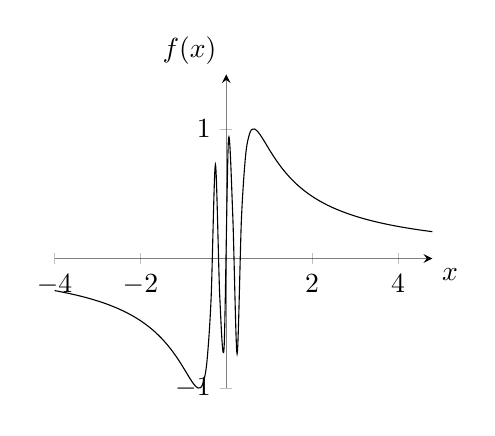
\begin{tikzpicture}
		\begin{axis}[scale=.7,draw opacity =.5,samples=100,smooth, 
		  axis x line=center, % no box around the plot, only x and y axis
		  axis y line=center, % the * suppresses the arrow tips
		  ylabel = {$f(x)$},
		  xlabel = {$x$},
		  xlabel style={below right},
		  ylabel style={above left},
		  xmin=-4,xmax=4,ymin=-1,ymax=1.2,
		  enlargelimits=upper] % extend the axes a bit to the right and top
		  \addplot[black,opacity=1]{sin(deg(1/x))};
		\end{axis}
	    \end{tikzpicture}
	    \end{center}
	    \vspace{.5cm}

	    Demostración.-\; Supongamos que existe algún $A\in \mathbb{R}$ tal que $\lim\limits_{x\to 0}f(x)=A.$ De la definición de límites esto significa que para todo $\epsilon>0$ existe un $\delta>0$ tal que 
	    $$|f(x)-A|<\epsilon\; \mbox{siempre que}\; 0<|x|<\delta$$
	    Primero, afirmamos que para cualquiera de estos $A$ debemos tener $|A|\leq 1$. Debe ser así porque si $|A|>1$ entonces $|A|-1>0$, de donde podríamos elegir $\epsilon$ tal que $0<\epsilon<(|A|-1)$. Pero se tiene $|f(x)|\leq 1$ para todo $x$, por consiguiente
	    $$|f(x)-A|=|A-f(x)|\geq |A|-|f(x)|\geq |A|-1>\epsilon$$
	    Esto contradice nuestra elección de $\epsilon$, por lo que $|A|$ deber ser menor o igual que 1.\\
	    Luego supongamos $|A|\leq 1$ y elegimos $\epsilon=\frac{1}{2}>0$. Para obtener nuestra contradicción debemos demostrar que no existe $\delta > 0$ tal que
	    $$|f(x)-A|<\dfrac{1}{2}\; \mbox{ siempre que } 0<|x|<\delta$$
	    Por la propiedad de Arquímedes de los números reales sabemos que para cualquier $x\in \mathbb{R}$, existe un entero positivo tal que $n$ con $n=1\; (modk\; 4)$. Pero,
	    $$0<\dfrac{2}{n\pi}<|x|\; \Longrightarrow \; 0<\dfrac{2}{(n+2)\pi}<|x|$$
	    Entonces, por la definición de $f$ y ya que $n=1\; (mod \;4)$ y $n+2=3\; (\mod\; 4)$, tenemos 
	    $$f\left(\dfrac{2}{n\pi}\right)=\sen\left(\dfrac{n\pi}{2}\right)=1 \qquad \quad f\left[\dfrac{2}{(n+2)\pi}\right]=\sen\left[\dfrac{(n+2)\pi}{2}\right]=-1$$
	    pero,
	    $$\bigg|f\left(\dfrac{n\pi}{2}\right)-A\bigg|\; \Longrightarrow \; |1-A|<\dfrac{1}{2} \; \Longrightarrow\; \dfrac{1}{2}<A\leq 1$$
	    Además,
	    $$\bigg|f\left[\dfrac{(n+2)\pi}{2}\right]-A\bigg|=|-1-A|>\dfrac{1}{2}.$$
	    Esto contradice que si $\lim\limits_{x\to 0}f(x)=A$ entonces para cada $\epsilon>0$ tenemos $|f(x)-A|<\epsilon$ para todo $0<|x|<\delta$. En otras palabras, encontramos un $\epsilon$ mayor que $0$ tal que no importa tan pequeño que elijamos $\delta$ existe un $x$ tal que $|x|$ es menor que $\delta$, pero $|f(x)-A|$ es mayor que $\epsilon$. Esto contradice la definición de $\lim\limits_{x\to 0}f(x)=A$. Por lo tanto no puede haber tal núemero en $A\in \mathbb{R}$.\\\\

    %-------------------- 28.
    \item Para $x\neq 0$, sea $f(x)=[1/x]$, designado por $[t]$ el mayor entero $\leq t.$ Trazar la gráfica de $f$ para los intervalos $[-2,-\frac{1}{5}]$ y $[\frac{1}{5},2]$. ¿Qué le ocurre a $f(x)$ cuando $x\to 0$ tomando valores positivos? ¿y tomando valores negativos? ¿Puede definirse $f(0)$ para que $f$ sea continuo en $0$? \\\\
	Respuesta.-\; 
	\begin{center}
	    \begin{tikzpicture}
	    \begin{axis}[scale=1.2,draw opacity =.5,samples=100,smooth, 
	      axis x line=center, 
	      axis y line=center,
	      ylabel = {$f(x)$},
	      xlabel = {$x$},
	      xlabel style={below right},
	      ylabel style={above left},
	      xmin=-2,xmax=2,ymin=-5,ymax=4,
	      label style={font=\tiny},
	      tick label style={font=\tiny},
	      enlargelimits=upper] 
	      \addplot[black,opacity=1,domain=-2:-1]{-1};
	      \addplot[fill=white,mark=*] coordinates {(-2,-1)};
	      \addplot[mark=*] coordinates {(-1,-1)};
	      \addplot[black,opacity=1,domain=-1:-.5]{-2};
	      \addplot[fill=white,mark=*] coordinates {(-1,-2)};
	      \addplot[mark=*] coordinates {(-.5,-2)};
	      \addplot[black,opacity=1,domain=-.5:-.35]{-3};
	      \addplot[fill=white,mark=*] coordinates {(-.5,-3)};
	      \addplot[mark=*] coordinates {(-.35,-3)};
	      \addplot[black,opacity=1,domain=-.35:-.25]{-4};
	      \addplot[fill=white,mark=*] coordinates {(-.35,-4)};
	      \addplot[mark=*] coordinates {(-.25,-4)};
	      \addplot[black,opacity=1,domain=-.25:-.15]{-5};
	      \addplot[fill=white,mark=*] coordinates {(-.25,-5)};
	      \addplot[mark=*] coordinates {(-.15,-5)};
	      \addplot[black,opacity=1,domain=.20:.25]{4};
	      \addplot[fill=white,mark=*] coordinates {(.2,4)};
	      \addplot[mark=*] coordinates {(.25,4)};
	      \addplot[black,opacity=1,domain=.25:.35]{3};
	      \addplot[fill=white,mark=*] coordinates {(.25,3)};
	      \addplot[mark=*] coordinates {(.35,3)};
	      \addplot[black,opacity=1,domain=.35:.5]{2};
	      \addplot[fill=white,mark=*] coordinates {(.35,2)};
	      \addplot[mark=*] coordinates {(.5,2)};
	      \addplot[black,opacity=1,domain=.5:1]{1};
	      \addplot[fill=white,mark=*] coordinates {(.5,1)};
	      \addplot[mark=*] coordinates {(1,1)};
	      \addplot[black,opacity=1,domain=1:2]{0};
	      \addplot[fill=white,mark=*] coordinates {(1,0)};
	      \addplot[mark=*] coordinates {(2,0)};
	    \end{axis}
	\end{tikzpicture}
	\end{center}
	\vspace{.5cm}
	Como $x\to 0^+,\; f(x)$ toma valores positivos arbitrariamente grandes.\\
	Como $x\to 0^-,\; f(x)$ toma valores negativos arbitrariamente grandes.\\
	No hay manera de definir $f(0)$ para que $f$ sea continuo en $0$.\\\\

    %-------------------- 29.
    \item Hacer lo mismo que en el ejercicio 28, cuando $f(x)=(-1)^{[1/x]}$ para $x\neq 0$.\\\\
	Respuesta.-\;
	\begin{center}
	    \begin{tikzpicture}
	    \begin{axis}[scale=1.2,draw opacity =.5,samples=100,smooth, 
	      axis x line=center, 
	      axis y line=center,
	      ylabel = {$f(x)$},
	      xlabel = {$x$},
	      xlabel style={below right},
	      ylabel style={above left},
	      xmin=-2,xmax=2,ymin=-1.5,ymax=1.5,
	      label style={font=\tiny},
	      tick label style={font=\tiny},
	      enlargelimits=upper] 
	      \addplot[black,opacity=1,domain=-2:-1]{-1};
	      \addplot[black,opacity=1,domain=-1:-.5]{1};
	      \addplot[black,opacity=1,domain=-.5:-.3]{-1};
	      \addplot[black,opacity=1,domain=-.3:-.23]{1};
	      \addplot[black,opacity=1,domain=-.23:-.2]{-1};

	      \addplot[black,opacity=1,domain=.2:.23]{1};
	      \addplot[black,opacity=1,domain=.23:.3]{-1};
	      \addplot[black,opacity=1,domain=.3:.5]{1};
	      \addplot[black,opacity=1,domain=.5:1]{-1};
	      \addplot[black,opacity=1,domain=1:2]{1};
	    \end{axis}
	\end{tikzpicture}
	\end{center}
	\vspace{.5cm}
	Como $x\to 0^+,\; f(x)$ alterna entre $1$ y $-1$.\\
	Como $x\to 0^-,\; f(x)$ alterna entre $1$ y $-1$.\\
	No hay forma  de definir $f(0)$ para que $f$ sea continuo en $0$, ya que $f(x)$ tomará ambos valores $1$ y $-1$ no importa cuán pequeño elijamos nuestro $\delta>0$.\\\\

    %-------------------- 30.
    \item Los mismo que en el ejercicio 28, cuando $f(x)=x(-1)^{[1/x]}$ para $x\neq 0$.\\\\
	Respuesta.-\;
	\begin{center}
	    \begin{tikzpicture}
	    \begin{axis}[scale=1,draw opacity =.5,samples=100,smooth, 
	      axis x line=center, 
	      axis y line=center,
	      ylabel = {$f(x)$},
	      xlabel = {$x$},
	      xlabel style={below right},
	      ylabel style={above left},
	      xmin=-2,xmax=2,ymin=-1.5,ymax=1.5,
	      label style={font=\tiny},
	      tick label style={font=\tiny},
	      enlargelimits=upper] 
	      \addplot[black,opacity=1,domain=-2:-1]{-x};
	      \addplot[black,opacity=1,domain=-1:-.5]{x};
	      \addplot[black,opacity=1,domain=-.5:-.37]{-x};
	      \addplot[black,opacity=1,domain=-.37:-.3]{x};
	      \addplot[black,opacity=1,domain=-.3:-.25]{-x};
	      \addplot[black,opacity=1,domain=.25:.3]{x};
	      \addplot[black,opacity=1,domain=.3:.37]{-x};
	      \addplot[black,opacity=1,domain=.37:.5]{x};
	      \addplot[black,opacity=1,domain=.5:1]{-x};
	      \addplot[black,opacity=1,domain=1:2]{x};
	    \end{axis}
	\end{tikzpicture}
	\end{center}
	\vspace{.5cm}
	Como $x\to 0^+$, $f(x)\to 0$.\\
	Como $x\to 0^-$, $f(x)\to 0$.\\
	Si definimos $f(0)=0$ entonces $f$ es continuo en $0$.\\\\

    %-------------------- 31.
    \item Dar un ejemplo de una función continua en un punto de un intervalo y discontinua en los demás puntos del intervalo, o probar que no existe una tal función.\\\\
	Demostración.-\; Sea $f$ una función en el intrevalo $[-a,a]$ tal que,
	$$f(x)=\left\{\begin{array}{rcl}
		x & \mbox{para} & x\in \mathbb{Q}\\
		-x & \mbox{para} & x\in \mathbb{R}\\
	\end{array}\right.$$
	Por lo tanto, la función $f$ es continua solo en el punto $x=0$, y discontinuo en todos los demás puntos del intervalo $[-a,a]$.\\\\

    %-------------------- 32.
    \item Sea $f(x)=x\sen (1/x)$ si $x\neq 0$. Definir $f(0)$ de manera que $f$ sea continua en $0$.\\\\
	Demostración.-\; Ya que $-1\leq \sen \dfrac{1}{x}\leq 1$ para todo $x\neq 0$ sabemos que,
	$$-x\leq x\sen\dfrac{1}{x}\leq x,\quad x\neq 0$$
	después se tiene que,
	$$\lim_{x\to 0}-x=\lim_{x\to 0}x=0$$
	Aplicando el teorema 3.3 concluimos,
	$$\lim_{x\to 0}x\sen\dfrac{1}{x}=0$$
	Por lo tanto, definiendo $f(0)=0$, extendemos $f$ a una función continua en $0$.\\\\

    %-------------------- 33.
    \item Sea $f$ una función tal que $|f(u)-f(v)|\leq |u-v|$ para todos los valores $u$ y $v$ de un intervalo $[a,b]$.

	    \begin{center}
		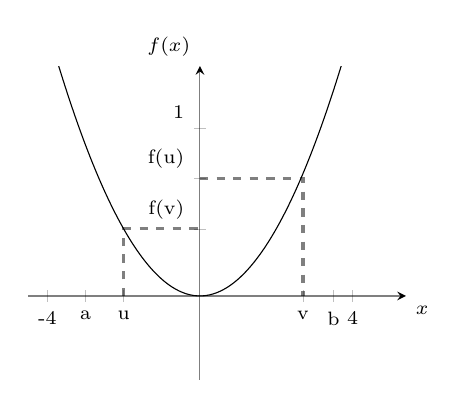
\begin{tikzpicture}
		\begin{axis}[scale=.7,draw opacity =.5,samples=100,smooth, 
		  axis x line=center, % no box around the plot, only x and y axis
		  axis y line=center, % the * suppresses the arrow tips
		  ylabel = {$f(x)$},
		  xlabel = {$x$},
		  xlabel style={below right},
		  ylabel style={above left},
		  label style={font=\scriptsize},
	          tick label style={font=\scriptsize},
		  yticklabel style={above left},
		  xtick={-4,-3,-2,2.7,3.5,4},
		  xticklabels={-4,a,u,v,b,4},
		  ytick={.7,.4,1},
		  yticklabels={f(u),f(v),1},
		  xmin=-4.5,xmax=4.5,ymin=-.5,ymax=1.2,
		  enlargelimits=upper] % extend the axes a bit to the right and top
		  \addplot[black,opacity=1]{x^2/10};
		  \addplot+[
		    black,very thick,dashed,
		    mark=none,
		    const plot,
		    empty line=jump,
		    ]
		    coordinates{
			(-2,0)
			(-2,.4)
			(0,.4)

			(0,.7)
			(2.7,.7)
			(2.7,0)
		    };
		\end{axis}
	    \end{tikzpicture}
	    \end{center}
	    \vspace{.5cm}

	\begin{enumerate}[\bfseries a)]

	    %---------- a)
	    \item Probar que $f$ es continua en cada punto de $[a,b]$.\\\\
		Demostración.-\; Sea $h$ cualquier punto en $[a,b]$, de donde para todo $\epsilon>0$ con $\delta=\epsilon$ se tiene por hipótesis que,
		$$|x-h|<\delta \;  \Longrightarrow \; |x-h|<\epsilon \; \Longrightarrow \; |f(x)-f(h)|<\epsilon$$
		Así, para todo $\epsilon>0$, tenemos $|f(x)-f(h)|<\epsilon$ siempre que $|x-h|<\delta$, y por lo tanto
		$$\lim_{x\to h}f(x)=f(h).$$\\\\


	    %---------- b)
	    \item Suponiendo que $f$ sea integrable en $[a,b]$, demostrar que
		$$\bigg|\int_a^b f(x)\; dx - (b-a)f(a)\bigg|\leq \dfrac{(b-a)^2}{2}$$
		Demostración.-\; Sea $x\in [a,b]$ tenemos,
		$$|f(x)-f(a)|\leq |x-a|=x-a$$
		y sabemos que,
		$$\int_a^b f(a)\; dx = (b-a)f(a)$$
		entonces,
		$$\begin{array}{rcl}
		    \bigg|\displaystyle\int_a^b f(x)\; dx - (b-a)f(a)\bigg|&=&\bigg|\displaystyle\int_a^b f(x)\; dx - \displaystyle\int_a^b f(a)\; dx\bigg|\\\\
									   &=&\bigg|\displaystyle\int_a^b \left[f(x)-f(a)\right]\; dx\bigg|\\\\
					 &\leq &\displaystyle\int_a^b|f(x)-f(a)|\; dx\\\\
					 &\leq &\displaystyle\int_a^b |x-a|\; dx = \int_a^b (x-a)\;dx\\\\
					 &=&\dfrac{x^2}{2}-ax\bigg|_a^b = \dfrac{(b-a)^2}{2}\\\\
		\end{array}$$
		\vspace{.5cm}

	    %---------- c)
	    \item Más general. Demostrar que para cualquier $c$ de $[a,b]$, se tiene
		$$\bigg|\int_a^b f(x)\; dx - (b-a)f(c)\bigg|\leq \dfrac{(b-a)^2}{2}$$
		Demostración.-\; Similar a la parte (b) se tiene que,
		$$\begin{array}{rcl}
		    \bigg|\displaystyle\int_a^b f(x)\; dx - (b-a)f(c)\bigg|&=&\bigg|\displaystyle\int_a^b f(x)\; dx - \displaystyle\int_a^b f(c)\; dx\bigg|\\\\
									   &\leq &\displaystyle\int_a^b|f(x)-f(c)|\; dx\\\\
									   &=&\displaystyle\int_a^b |x-c|\; dx\\\\
		\end{array}$$
		Luego ya que $c\in [a,b]$ y $|x-a|=-(x-c)$ para $x<c$ y $|x-c|=x-c$ para $x\geq c$,
		$$\begin{array}{rcl}
		    \displaystyle\int_a^b|x-c|\; dx&=&\displaystyle\int_a^c -(x-c)\; dx + \int_c^b (x-c)\; dx\\\\
						   &=&-\dfrac{x^2}{2}\bigg|_a^c +c\cdot x\bigg|_a^c +\dfrac{x^2}{2}\bigg|_c^b - c\cdot x\bigg|_c^b\\\\
						   &=&\dfrac{a^2-c^2}{2}+c(c-a)+\dfrac{b^2-c^2}{2} - c(b-c)\\\\
						   &=&\dfrac{a^2+b^2}{2}+c^2-c(b+a)\\\\
		\end{array}$$
		Pero, sabemos que $c\in[a,b]$ implica que $c\leq b$ por lo que 
		$$\begin{array}{rcl}
		    \dfrac{a^2+b^2}{2}+c^2-c(b+a)&=&\dfrac{a^2+b^2}{2}+c[c-(b+a)]\\\\
		    &\leq&\dfrac{b^2+a^2}{2}+b(b-b-a)\\\\
		    &=&\dfrac{b^2+a^2}{2}-ab\\\\
		    &=&\dfrac{b^2-2ab+a^2}{2}\\\\
		    &=&\dfrac{(b-a)^2}{2}\\\\
		\end{array}$$

	\end{enumerate}

\end{enumerate}

\end{comment}

\section{funciones compuestas y continuas}

\begin{tcolorbox}
    \begin{def.}
	Sean $u$ y $v$ dos funciones dadas cualquiera. La compuesta o la composición de $u$ y $v$ en ese orden se define como la función $f$ para la cual
	$$f(x)=u[v(x)]$$
	Es decir, para calcular el valor de $f$ en $x$ primero se calcula $v(x)$ y luego se calcula $u$ e el punto $v(x)$. Naturalmente que para que este cálculo tenga sentido, es necesario que los valores de $v(x)$ entren en el dominio de la función $u$, y $f$ estará sólo definida en aquellos puntos $x$ para los cuales $v(x)$ está en el dominio de $u$.
    \end{def.}
\end{tcolorbox}

La notación para indicar composición es: 
$$f=u\circ v$$
que tiene una analogía con la notación de producto $u\cdot v$. En efecto, se verá a continuación que la operación de composición tiene algunas de las propiedades de la multiplicación
La \textbf{ley asociativa} está dada por:
$$u\circ(v\circ w) = (u\circ v)\circ w$$
La demostración  inmediata. Luego la ley conmutativa no es siempre válida en la composición.\\

\begin{teo}
    Suponiendo que $v$ continua en $p$ y que $u$ es continua en $q$, siendo $q=v(p)$, la función compuesta $f=u\circ v$ es continua en $p$.\\\\
	Demostración.-\; Puesto que $u$ es continua en $q$, para todo entorno $N_1[u(q)]$ existe un entorno $N_2(q)$ tal que 
	$$u(y)\in N[u(q)]\mbox{ siempre que } y \in N_2(q).$$
	Pero $q=v(p)$ y $v$ es continua en $p$, de modo que para el entorno $N_2(q)$ existe otro entorno $N_3(p)$ tal que 
	$$v(x)\in N_2(q)\mbox{ siempre que } x\in N_3(p).$$
	Si ponemos $y=v(x)$ y combinamos estas últimas, encontramos que para todo entorno $N_1(u[v(p)])$ existe un entorno $N_3(p)$ tal que 
	$$u[v(x)]\in N_1[f(p)]\mbox{ siempre que } x\in N_3(p),$$
	o, dicho de otro modo, puesto que $f(x)=u[v(x)],$
	$$f(x)\in N_1[f(p)]\mbox{ siempre que } x\in N_3(p).$$
	Esto significa que $f$ es continua en $p$, como se afirmó.\\\\

\end{teo}

\section{Ejercicios}

En los Ejercicios del $1$ al $10$, las funciones $f$ y $g$ están definidas por las fórmulas dadas. Si no se dice lo contrario, los dominios de $f$ y $g$ consisten en todos los números reales. Pongamos $h(x)=f[g(x)]$ siempre que $g(x)$ esté en el dominio de $f$. En cada caso, precisar el dominio de $h$ y dar una o más fórmulas para la determinación de $h(x)$.\\

\begin{enumerate}[\bfseries 1.]

    %-------------------- 1.
    \item $f(x)=x^2-2x, \qquad g(x)=x+1$.\\\\
	Respuesta.- Sea $h(x)=f[g(x)]$ entonces,
	$$h(x)=(x+1)^2-2x = x^2+2x+1-2x = x^2+1$$
	esto es válido para $x\in \mathbb{R}$.\\\\


    %-------------------- 2.
    \item $f(x)=x+1, \qquad g(x)=x^2-2x$.\\\\
	Respuesta.- Sea $h(x)=f[g(x)]$ entonces,
	$$h(x)=x^2-2x+1 = (x-1)^2$$
	válido para $x\in \mathbb{R}$.\\\\

    %-------------------- 3.
    \item $f(x)=\sqrt{x},$ si $x\leq 0 \qquad g(x)=x^2.$\\\\
	Respuesta.- Sea $h(x)=f[g(x)]$ entonces,
	$$h(x)=\sqrt{x^2}=|x|.$$
	Ya que $g(x)\geq 0$ la composición es válida para todos $x\in \mathbb{R}$.\\\\

    %-------------------- 4.
    \item $f(x)=\sqrt{x}$ si $x\geq 0, \qquad g(x)=-x^2$.\\\\
	Respuesta.- Sea $h(x)=f[g(x)]$ entonces,
	$$h(x)=\sqrt{-x^2}$$
	Ya que $-x^2\leq 0$ y $\sqrt{x}\geq 0$ la composición sólo está definida para $x=0$.\\\\

    %-------------------- 5.
    \item $f(x)=x^2,\qquad g(x)=\sqrt{x}$ si $x\geq 0.$\\\\
	Respuesta.- Sea $h(x)=f[g(x)]$ entonces,
	$$h(x)=\left(\sqrt{x}\right)^2=x.$$
	Esto es válido para $x\geq 0$.\\\\

    %-------------------- 6.
    \item $f(x)=-x^2,\qquad g(x)=\sqrt{x}$ si $x\geq 0.$\\\\
	Respuesta.- Sea $h(x)=f[g(x)]$ entonces,
	$$h(x)=-\left(\sqrt{x}\right)^2=-x.$$
	Esto es válido para $x\geq 0$.\\\\

    %-------------------- 7.
    \item $f(x)=\sen x,\qquad g(x)=\sqrt{x}$ si $x\geq 0.$\\\\
	Respuesta.- Sea $h(x)=f[g(x)]$ entonces,
	$$h(x)=\sen \left(\sqrt{x}\right).$$
	Es válido para $x\geq 0$.\\\\

    %-------------------- 8.
    \item $f(x)=\sqrt{x}$ si $x\geq 0,\qquad g(x)=\sen x$.\\\\
	Respuesta.- Sea $h(x)=f[g(x)]$ entonces,
	$$h(x)=\sqrt{\sen x}.$$
	Es válido para $x\geq 0$, por el hecho de que se define el dominio de $f$ como $x\geq 0$.\\\\

    %-------------------- 9.
    \item $f(x)=\sqrt{x}$ si $x>0,\qquad g(x)=x+\sqrt{x}$ si $x>0$.\\\\
	Respuesta.- Sea $h(x)=f[g(x)]$ entonces,
	$$h(x)=\sqrt{x+\sqrt{x}}.$$
	Ya que $g(x)=x+\sqrt{x}>0$ y $f$ está definida en $x>0$, la composición es válida para $x>0$.\\\\

    %-------------------- 10.
    \item $f(x)=\sqrt{x+\sqrt{x}}$ si $x>0, \qquad g(x)=x+\sqrt{x}$ si $x>0$.\\\\
	Respuesta.- Sea $h(x)=f[g(x)]$ entonces,
	$$h(x)=\sqrt{x+\sqrt{x}+\sqrt{x+\sqrt{x}}}$$
	Ya que cada función está definida par $x>0$, entonces la composición es válida para $x>0$.\\\\

Calcular los límites en los ejercicios del 11 al 20 y explicar qué teoremas se aplican en cada caso.\\\\

    %-------------------- 11.
    \item $\lim\limits_{x\to -2} \dfrac{x^3+8}{x^2-4}$.\\\\
	Respuesta.-\; $$\lim\limits_{x\to -2} \dfrac{x^3+8}{x^2-4} = \lim_{x\to -2}\dfrac{(x+2)(x^2-2x+4)}{(x+2)(x-2)} = \lim_{x\to 0}\dfrac{x^2-2x+4}{x-2} = -3$$\\

    %-------------------- 12.
    \item $\lim\limits_{x\to 4}\sqrt{1+\sqrt{x}}.$\\\\
	Respuesta.-\; $$\lim\limits_{x\to 4}\sqrt{1+\sqrt{x}} = \sqrt{3}.$$\\

    %-------------------- 13.
    \item $\lim\limits_{t\to 0}\dfrac{\sen(\tan t)}{\sen t}.$\\\\
	Respuesta.-\; Recordemos que $\lim\limits_{x\to 0}\dfrac{\sen x}{x}=1$, por lo tanto
	$$\lim_{t\to 0}\dfrac{\sen(\tan t)}{\sen t}=\lim_{t\to 0} \left(\dfrac{1}{\cos t}\cdot \dfrac{\sen(\tan t)}{\dfrac{\sen t}{\cos t}}\right) = \lim_{t\to 0}\left(\dfrac{1}{\cos t}\cdot \dfrac{\sen(\tan t)}{\tan t}\right) = \lim_{t\to 0}\dfrac{1}{\cos t}\cdot \lim_{t\to 0}\dfrac{\sen (\tan t)}{\tan t} = 1.$$\\

    %-------------------- 14.
    \item $\lim\limits_{x\to \pi/2} \dfrac{\sen(\cos x)}{\cos x}$.\\\\
	Respuesta.-\; Sean $\lim\limits_{x\to \pi/2} \cos x = \cos \dfrac{\pi}{2} = 0\; $ y $\; \lim\limits_{x\to 0}\dfrac{\sen x }{x} = 1$ entonces
	$$\lim_{x\to \pi/2}\dfrac{\sen(\cos x)}{\cos x}=1.$$\\


    %-------------------- 15.
    \item $\lim\limits_{t\o \pi}\dfrac{\sen(t-\pi)}{t-\pi}$.\\\\
	Respuesta.-\; Sea $x=t-\pi$, donde $t\to \pi$ es $x \to 0$ entonces,
	$$\lim\limits_{t\to \pi}\dfrac{\sen(t-\pi)}{t-\pi} = \lim\limits_{x\to 0}\dfrac{\sen x}{x}=1.$$\\

    %-------------------- 16.
    \item $\lim\limits_{x\to 1}\dfrac{\sen(x^2-1)}{x-1}$.\\\\
	Respuesta.-\; Sea $\lim\limits_{x\to 0}\dfrac{\sen x}{x}=1$ entonces,
	$$\lim_{x\to 1}\dfrac{\sen(x^2-1)}{x-1} = \lim_{x\to 1}\left[x+1\cdot \dfrac{\sen(x^2-1)}{(x+1)(x-1)}\right] = \lim_{x\to 1} (x + 1)\cdot \lim_{x\to 1}\dfrac{\sen(x^2-1)}{x^2-1} = 2.$$\\

    %-------------------- 17.
    \item $\lim\limits_{x\to 0} x\sen \dfrac{1}{x}$.\\\\
	Respuesta.-\; Ya que $\lim\limits_{x\to 0} f(x)=f(0)$ y $$-1\leq \sen \dfrac{1}{x}\leq 1,\; x\neq 0 \; \Longrightarrow \; -x\leq x\sen \dfrac{1}{x}\leq x,\; x\neq 0$$ 
	como también,
    $$\lim_{x\to 0} -x = 0\qquad y \qquad \lim_{x\to 0} x = 0$$
    entonces por el teorema 3.3 concluimos que,
    $$\lim_{x\to 0} x\sen \dfrac{1}{x}=0.$$\\


    %-------------------- 18.
    \item $\lim\limits_{x\to 0}\dfrac{1-\cos 2x}{x^2}$.\\\\
	Respuesta.-\; Sea $\cos(2x)=1-2\sen^2 x$ entonces,
	$$\lim_{x\to 0}\dfrac{1-\cos(2x)}{x^2} = \lim_{x\to 0}\dfrac{1-(1-2\sen^2 x)}{x^2} = 2\cdot \lim_{x\to 0}\dfrac{\sen^2 x}{x^2} = \lim_{x\to 0}\dfrac{\sen x}{x}\cdot \lim_{x\to 0}\dfrac{\sen x}{x} =  2.$$\\

    %-------------------- 19.
    \item $\lim\limits_{x\to 0} \dfrac{\sqrt{1+x}-\sqrt{1-x}}{x}$.\\\\
	Respuesta.-\; 
	$$\begin{array}{rcl}
	    \lim\limits_{x\to 0}\dfrac{\sqrt{1-x}-\sqrt{1-x}}{x}&=&\lim\limits_{x\to 0}\dfrac{\left(\sqrt{1+x}-\sqrt{1-x}\right)\left(\sqrt{1+x}+\sqrt{1-x}\right)}{x\left(\sqrt{1+x}+\sqrt{1-x}\right)}\\\\
								&=&\lim\limits_{x\to 0}\dfrac{(1+x)-(1-x)}{x\left(\sqrt{1+x}+\sqrt{1-x}\right)}\\\\
								&=&\lim\limits_{x\to 0}\dfrac{2}{\sqrt{1+x}+\sqrt{1-x}}\\\\
								&=&1.\\\\

	\end{array}$$

    %-------------------- 20.
    \item $\lim\limits_{x\to 0} \dfrac{1-\sqrt{1-4x^2}}{x^2}$.\\\\
	Respuesta.-\;
	$$\begin{array}{rcl}
	    \lim\limits_{x\to 0}\dfrac{1-\sqrt{1-4x^2}}{x^2}&=&\lim\limits_{x\to 0}\dfrac{\left(1-\sqrt{1-4x^2}\right)\left(1+\sqrt{1-4x^2}\right)}{x^2\left(1+\sqrt{1-4x^2}\right)}\\\\
							    &=&\lim\limits_{x\to 0}\dfrac{1-(1-4x^2)}{x^2\left(1+\sqrt{1-4x^2}\right)}\\\\
							    &=&\lim\limits_{x\to 0}\dfrac{4}{1-\sqrt{1-4x^2}}\\\\
					  &=&2.\\\\
	\end{array}$$

    %-------------------- 21.
    \item 

\end{enumerate}



